% Kepler effective potential J^2/(2 m r^2)-alpha/r.
% Reference: handdraw/Veff.png. Scaled units: J^2/(m alpha)=2.
% Compile: pdflatex Veff_tikz.tex
\documentclass[tikz,border=6pt]{standalone}
\usepackage{amsmath}
\usepackage{fix-cm}
\usetikzlibrary{arrows.meta}
\begin{document}
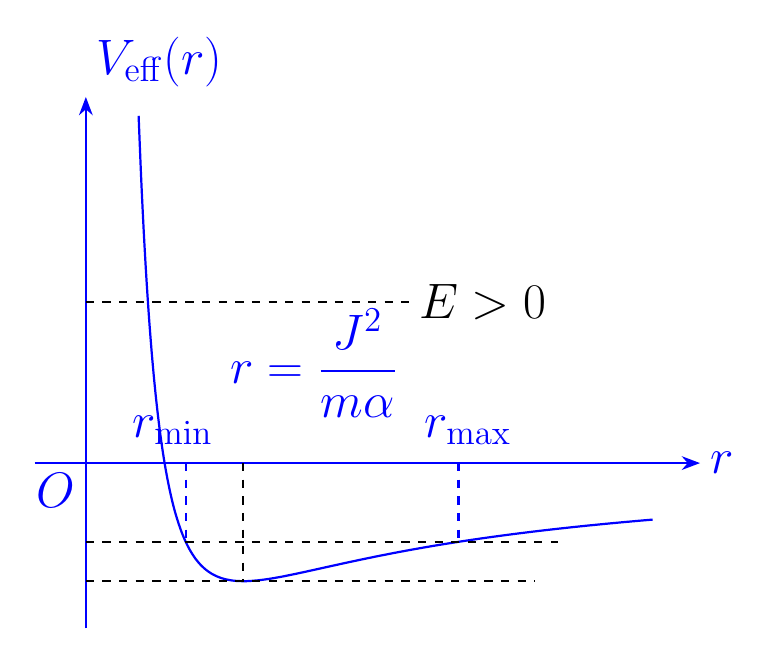
\begin{tikzpicture}[>=Stealth,thick,every node/.style={font=\fontsize{18}{22}\selectfont}]
  \draw[blue,->] (-.65,0) -- (7.8,0) node[right] {$r$};
  \draw[blue,->] (0,-2.1) -- (0,4.65) node[above right] {$V_{\mathrm{eff}}(r)$};
  \node[blue,below left] at (0,0) {$O$};
  \draw[blue,domain=.67:7.2,samples=200,smooth] plot (\x,{6*(1/(\x*\x)-1/\x)});
  % E=-1 gives r_min=3-sqrt(3), r_max=3+sqrt(3); the minimum is -1.5.
  \draw[dashed] (0,2.05) -- (4.1,2.05) node[right] {$E>0$};
  \draw[dashed] (0,-1) -- (6,-1);
  \draw[dashed] (0,-1.5) -- (5.7,-1.5);
  \draw[blue,dashed] ({3-sqrt(3)},0) -- ({3-sqrt(3)},-1);
  \draw[dashed] (2,0) -- (2,-1.5);
  \draw[blue,dashed] ({3+sqrt(3)},0) -- ({3+sqrt(3)},-1);
  \node[blue,above] at (1.10,.10) {$r_{\min}$};
  \node[blue,above] at (4.85,.10) {$r_{\max}$};
  \node[blue,above] at (2.9,.45) {$r=\dfrac{J^2}{m\alpha}$};
\end{tikzpicture}
\end{document}
